\chapter{Wykorzystane algorytmy i ich charakterystyka}
\label{chap:Algorytmy}
\textit{Autor: Bartosz Kołakowski}
\setlength{\parindent}{0pt}
\section{Base64}
\label{sec:Base64}
\subsection{Opis Base64}
\label{sec:Base64Opis}
Podczas przesyłania danych przez sieć pojawił się u nas problem, że na przykład podpis cyfrowy czy klucz publiczny są w postaci ciągu bajtów. Ich przesyłanie przez sieć w bezpośredniej formie jest dość problematyczne, więc dobrym rozwiązaniem problemu jest ich przekonwertowanie na format danych jaki ma łańcuch znaków. Można bezpośrednio dekodować bajt po bajcie na ich odpowiednik w formacie UTF-8, lecz przez nas został wybrany bardzo uniwersalny i powszechnie znany format Base64, który dzieli ciąg bajtów na trzy-bajtowe grupy, które są potem dzielone na cztery sześciobitowe grupy, a każdy z tych zestawów sześciobitowych jest zamieniany na jedną liczbę mnożąc bity od najmłodszego do najstarszego przez kolejną potęgę liczby dwa według wzoru:
\begin{equation}
    Liczba = \sum_{i=1}^6 bit_i * 2^{i-1}
\end{equation}
Podział ciągu bajtów na trzy-bajtowe grupy, na następnie na cztery sześciobitowe grupy został zwizualizowany, na poniższej grafice:
\begin{figure}[H]
    \centering
    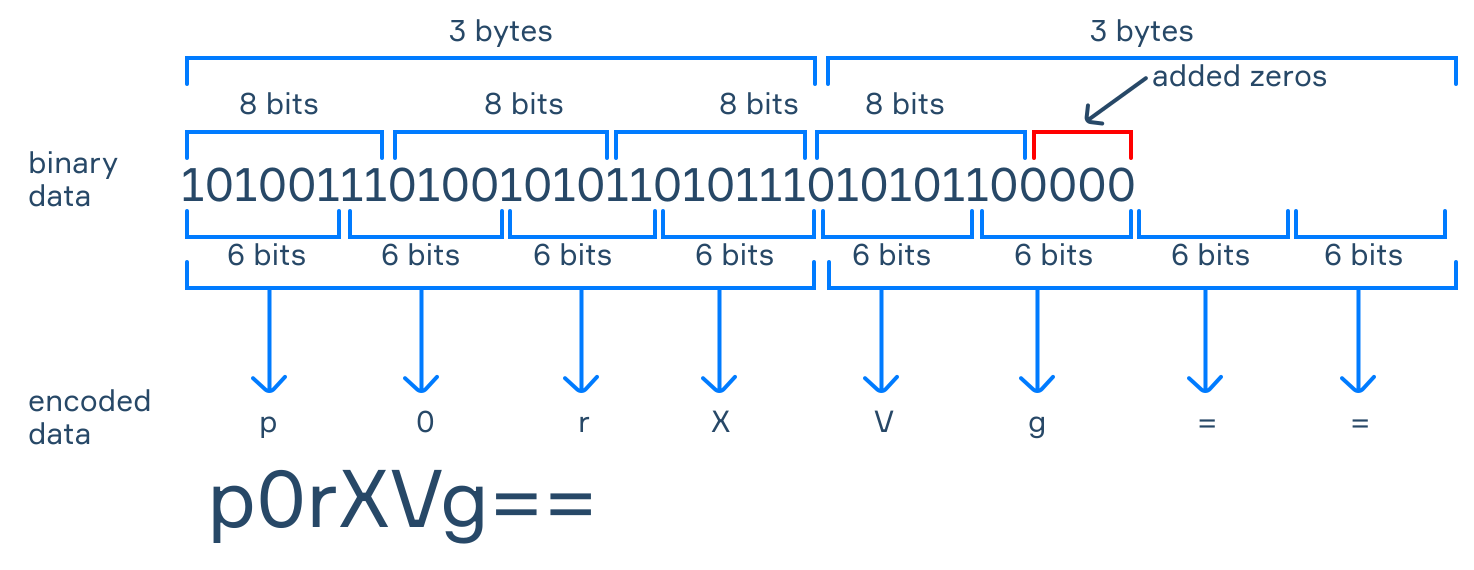
\includegraphics[width=\textwidth]{Images/Base64Schema.png}
    \caption{Schemat Base64}
	\label{fig:Base64Schema}
\end{figure}
Potem ta liczba konwertowana jest na jeden z sześćdziesięciu czterech znaków ASCII (jest to albo cyfra od 0 do 9, albo wielka litera od A do Z, albo mała litera od a do z albo znak plusa lub równości). Odbywa się to zgodnie ze schematem pokazanym na poniższym obrazku:
\begin{figure}[H]
    \centering
    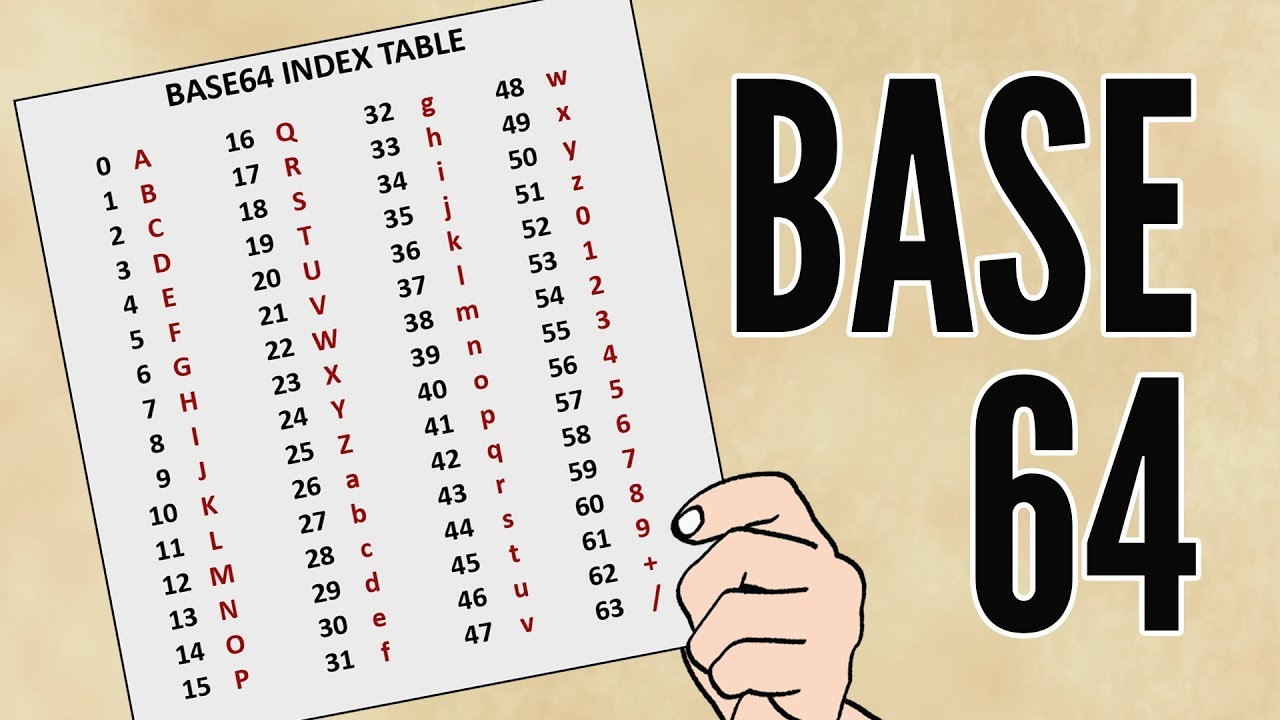
\includegraphics[width=\textwidth]{Images/Base64Coding.jpg}
    \caption{Kodowanie w Base64}
	\label{fig:Base64Coding}
\end{figure}
Potem po otrzymaniu ciągu znaków w formacie Base64 można go łatwo odkodować na ciąg bajtów, gdyż algorytm jest powszechnie znany i problem z odszyfrowaniem jaki ciąg bitów jest reprezentowany przez dany znak nie występuje.

\vspace{1em}

Dodatkowo, jeśli długość ciągu bajtów nie jest liczbą podzielną przez trzy stosuje się metodę zwaną dopełnieniem, która zamiast wcześniej opisanych znaków dodaje znaki równa się tak, żeby liczba znaków po konwersji była liczbą podzielną przez cztery.

\vspace{1em}

Istnieją również alternatywy do Base64, oparte na podobnych założeniach takie jak Base62, Base36, Base32 czy Base16. Base64 został przez nas wybrany, ponieważ wśród wszystkich tych algorytmów jest najbardziej efektywny.
\subsection{Użycie Base64 w praktyce}
\label{chap:Base64Praktyka}
\begin{lstlisting}
self.EncryptedKString = base64.b64encode(self.EncryptedKBytes).decode('utf-8')
\end{lstlisting}
\begin{lstlisting}
base64.b64encode(self.EncryptedKBytes).decode('utf-8')
\end{lstlisting}
Korzystano z funkcji b64encode występującej w bibliotece Base64 by przekonwertować dane w postaci binarnej na format Base64 (potem jeszcze zamieniane jest to na format tekstowy UTF-8).
\section{Podpis cyfrowy}
\label{sec:PodpisCyfrowy}
\subsection{Opis podpisu cyfrowego}
\label{sec:PodpisCyfrowyOpis}
Podczas sytuacji, kiedy nasz zestaw wiadomości został zweryfikowany jako prawidłowy i teraz pozostaje kwestia jak zabezpieczyć blok przed nieautoryzowanymi zrachowaniami (zmianami treści wiadomości), tak aby każdy członek sieci mógł w łatwy sposób sprawdzić czy faktycznie, nikt nie zmodyfikował wiadomości (na przykład w celu oszustwa, które ma mu przynieść korzyść).

\vspace{1em}

W metodzie konsensusu proof-of-work poprawność bloku sprawdza się poprzez porównywanie funkcji skrótu odpowiednio ze sobą połączonych bloków. Wadą tego rodzaju rozwiązania jest fakt, że do samego sprawdzenia podpisu potrzebne są ogromne moce obliczeniowe, co jest mocno nie korzystne i dodatkowo jednostka lub zespół jednostek posiadający odpowiednio dużą moc obliczeniową może zamienić treści wiadomości w poprzednich blokach w łańcuchu tak, aby wartość funkcji skrótu się zgadzała z nowszymi wiadomościami i nie wzbudzała podejrzeń.

\vspace{1em}

Tak łączone są bloki w Proof Of Work za pomocą funkcji skrótów:
\begin{figure}[H]
    \centering
    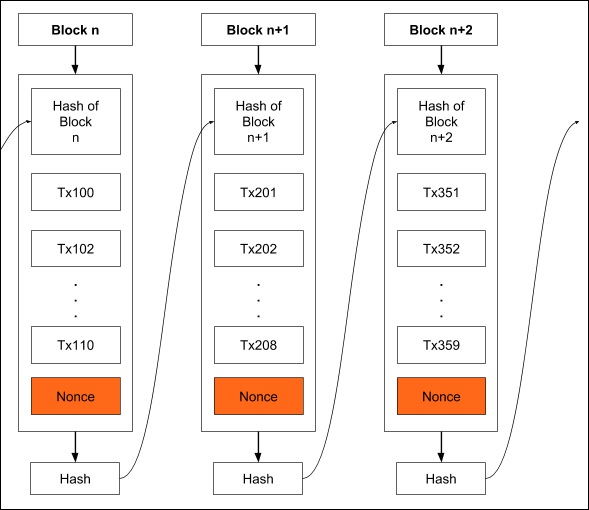
\includegraphics[width=\textwidth]{Images/ProofOfWorkHash.jpg}
    \caption{Działanie funkcji skrótu w Proof Of Work}
    \label{fig:ProofOfWorkHash}
\end{figure}

My zamiast stosować skomplikowany zestaw połączonych ze sobą funkcji skrótu postanowiliśmy skorzystać z innego rozwiązania znanego z zastosowań kryptograficznych. Jest to podpis cyfrowy, ale zanim przejdę do omówienia jego i jego charakterystyki warto pokazać na przykładzie jakie rozwiązania są w nim stosowane, a jakie nie i dlaczego.

\vspace{1em}

W kryptografii asymetrycznej każdy z użytkowników ma dwa klucze – klucz publiczny i klucz prywatny. Jeśli weryfikator z wiadomości znajdujących się w bloku wygenerowałby wartość z funkcji skrótu i próbował podpisać ją kluczem publicznym to przecież żaden z użytkowników nie miałby możliwości zweryfikowania takiego podpisu, ponieważ do to tego potrzebny jest drugi klucz, czyli klucz prywatny, ale na tym polega cała kryptografia asymetryczna, że klucz prywatny jest niedostępny dla innych.

\vspace{1em}

Schematyczne zilustrowanie podpisu cyfrowego:
\begin{figure}[H]
    \centering
    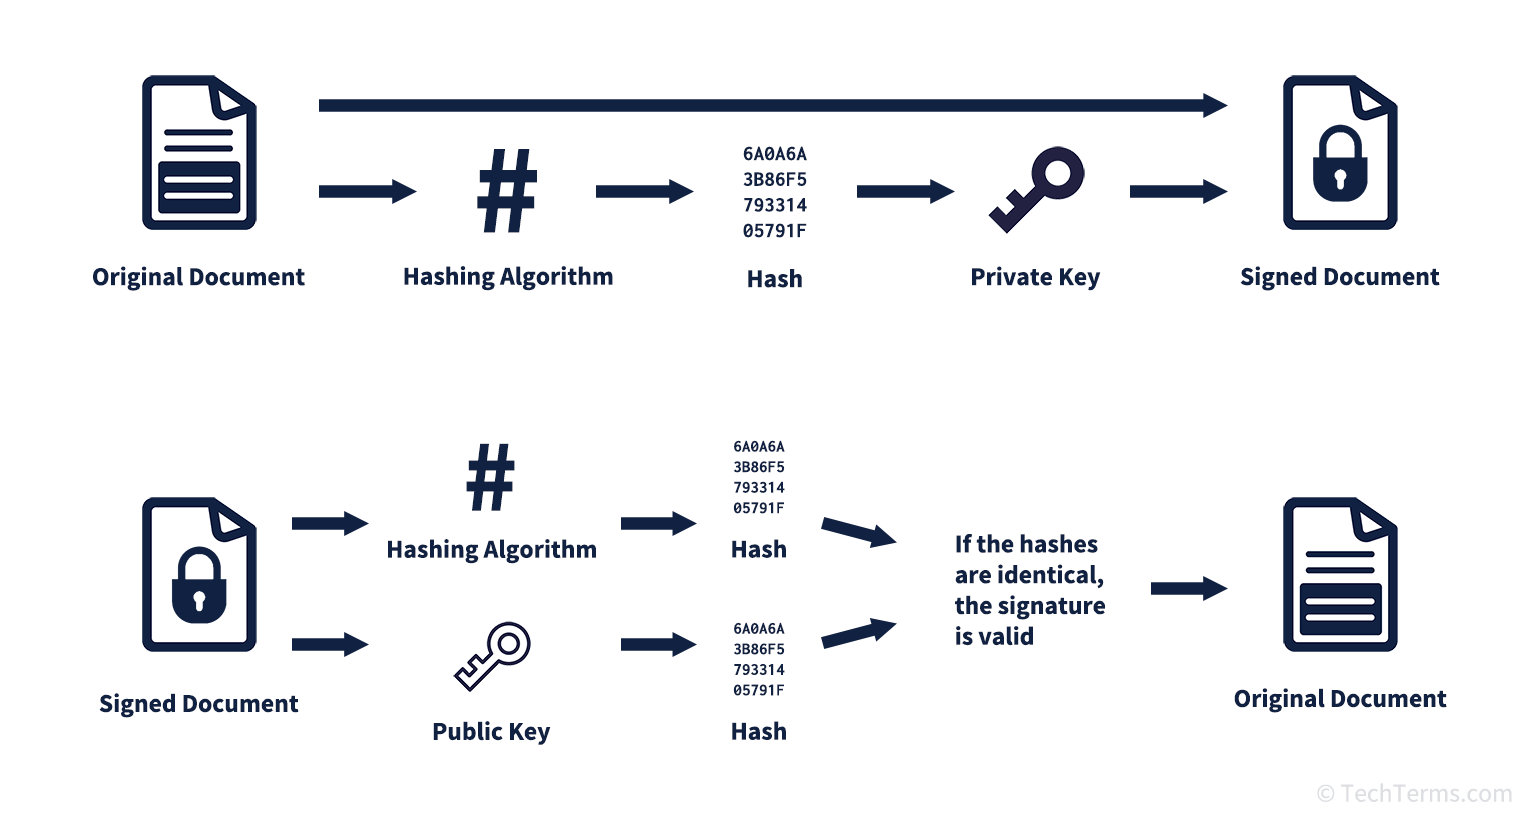
\includegraphics[width=\textwidth]{Images/DSJPG.jpg}
    \caption{Działanie podpisu cyfrowego}
    \label{fig:DSJP}
\end{figure}
Z tego powodu, żeby wykonać operację podpisu cyfrowego potrzebujemy mieć wiadomości z bloku danych wykonać na nich operację funkcji skrótu (tu wykorzystywany jest SHA-256) po czym wykonujemy podpis cyfrowy z użyciem klucza prywatnego i konwertujemy ciąg bajtów na łańcuch tekstowy za pomocą Base64.
\subsection{Użycie podpisu cyfrowego w praktyce}
\label{sec:PodpisCyfrowyPraktyka}
\begin{lstlisting}
def sendDigitalSignature(self, ListOfJSON, me):
    jsonMessages = self.get_messages_block(ip())
    drawnVerifier = self.drawVerifier()
    print("Drawn Verifier " + str(drawnVerifier))
    if drawnVerifier == self.port:
        me.remove_single_message_JSON(ip())
        for count, jsonSingleMessage in enumerate(jsonMessages):
            if jsonMessages[count] == ListOfJSON[0]:
                length = len(ListOfJSON)
                identicalResult = jsonMessages[count:count+length]
                                == ListOfJSON
                if identicalResult:
                    jsonAString = json.dumps(ListOfJSON, sort_keys=True,
                    separators=(',', ':'))
\end{lstlisting}
Jeżeli dany użytkownik został wylosowany jako weryfikator, a następnie jeśli otrzymane wiadomości (od osoby wysyłającej ostatnią wiadomość w bloku) zgadzają się z wiadomościami, które posiada weryfikator to potwierdza je on za pomocą wystawienia podpisu cyfrowego.
\begin{lstlisting}
def createSignature(self, dataStrng):
    data = dataStrng.encode('utf-8')
    signature = self.private_key.sign(
        data,
        padding.PKCS1v15(),
        hashes.SHA256()
    )
    return signature
\end{lstlisting}
Następnie tworzymy podpis cyfrowy na podstawie przekazanych wiadomości w formie łańcucha znaków. Jest to szczegółowo robione tak, że łańcuch znaków przekształcany jest do postaci binarnej, potem te dane binarne są podpisywane przy wykorzystaniu klucza prywatnego (dlaczego klucza prywatnego, a nie publicznego zostało wcześniej wyjaśnione). Poza samymi danymi innymi argumentami w schemacie podpisu cyfrowego jest wypełnienie (angielski – padding) – tu używane jest schemat PKCS1v15. Innym argumentem do funkcji podpisu cyfrowego jest określona funkcja skrótu, ponieważ podpisywanie całego ciągu znaków binarnych byłoby zbyt czasochłonne, w tym przypadku zastosowano algorytm SHA256.

\vspace{1em}

Pojawia się pytanie czy każdy z użytkowników będzie mógł dla tych samych danych otrzymać taki sam podpis cyfrowy i czy przy weryfikacji podpisu cyfrowego dla tych samych danych otrzyma ten sam wynik. Jest to kluczowe dla działania programu, jeśli to nie zostałoby zapewnione weryfikacji podpisu cyfrowego byłaby nie możliwa. Pożądana przez nas cecha algorytmu, czyli fakt, że dla tych samych danych algorytm zawsze zwróci ten sam wynik to deterministyczność. Jak sprawdzić czy nasz podpis cyfrowy jest deterministyczny – trzeba dowiedzieć się czy funkcja privateKey.sign zwraca deterministyczny wynik, a faktem jest informacja, że w tej funkcji jest to uzależnione od tego jakie wypełnienie jest stosowane oraz jaki algorytm generowania funkcji skrótu jest stosowany. Co do metody wypełnienia PKCS1v15 – jest ona deterministyczna (nie stosuje ona elementów losowanych w przeciwieństwie do wielu innych metod wypełnienia), funkcja skrótu SHA256 (w przeciwieństwie do niektórych innych funkcji skrótu) jest deterministyczna. Ukazując, to że metoda wypełnienia jak i funkcja skrótu są deterministyczne, wskazujemy na to, że funkcja generująca podpis cyfrowy, która od nich bezpośrednio zależy również jest deterministyczna, więc udowodniliśmy, że podpis cyfrowy jest deterministyczny (taki sam dla identycznych danych wejściowych).
\begin{lstlisting}
def createSignatureBase64(self, dataStrng):
    bytesSignature = self.createSignature(dataStrng)
    return base64.b64encode(bytesSignature).decode('utf-8')
\end{lstlisting}
Tu stworzony podpis cyfrowy w formie ciągu bajtów konwertujemy na łańcuch znaków przy użyciu Base64 (którego działanie opisano w innym akapicie) i dekodujemy na format UTF-8, tak aby dało się go wysłać komfortowo przez sieć.
\begin{lstlisting}
if identicalResult:
    jsonAString = json.dumps(ListOfJSON, sort_keys=True, separators=(',', ':'))
    base64Signature = self.createSignatureBase64(jsonAString)
    requests.post("http://{}:{}/send_message".format(ip(), self.port),
      json={"addr": ip(), "port": self.port,
            "message": "-----BEGIN DIGITAL SIGNATURE-----\n*" + 
            str(drawnVerifier) + "*" + base64Signature + "\n"})
    for peer in self.peers:
        requests.post("http://{}:{}/send_message".format(peer.addr, peer.port),
          json={"addr": peer.addr, "port": peer.port,
                "message": "-----BEGIN DIGITAL SIGNATURE-----\n*" + 
                str(drawnVerifier) + "*" + base64Signature + "\n"})
\end{lstlisting}
Potem mając już gotowy podpis cyfrowy przesyłamy go innym użytkownikom, przed samym podpisem dodając odpowiedni nagłówek, tak aby odbiorcy mieli większą łatwość w jego odczytaniu.
\begin{figure}[H]
    \centering
    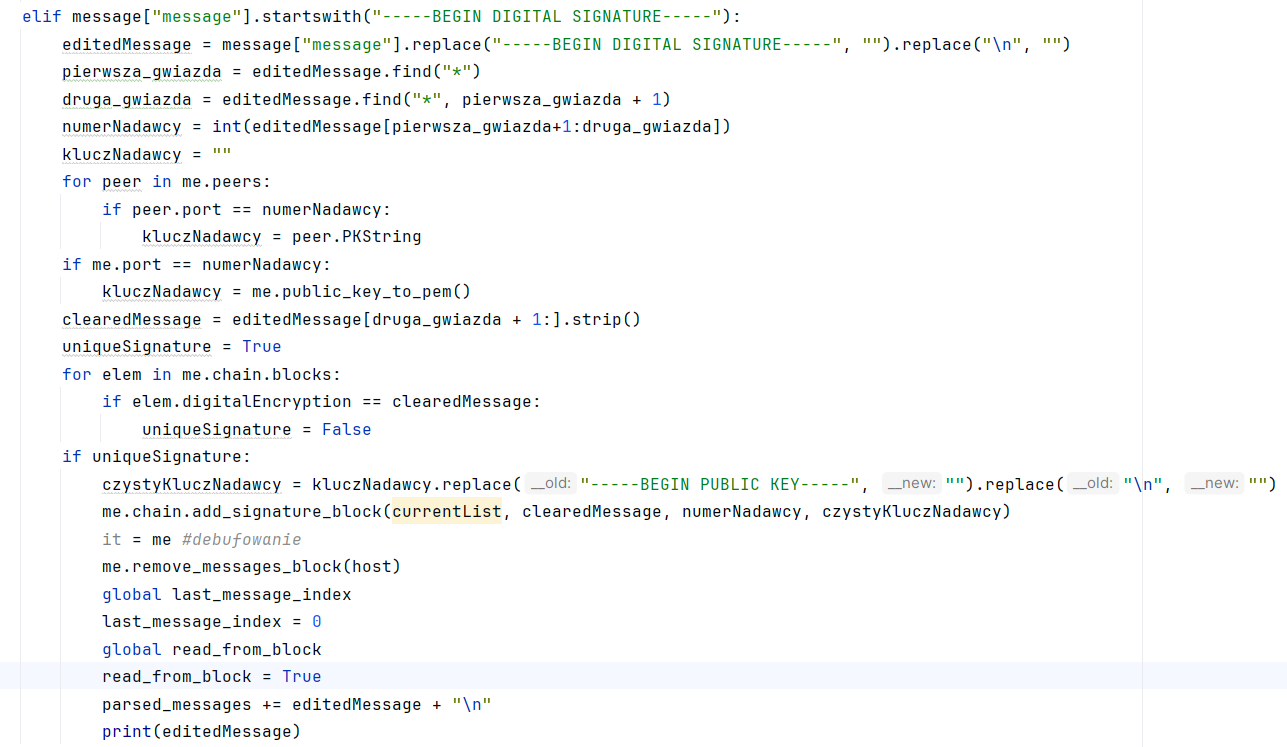
\includegraphics[width=\textwidth]{Images/Code7.png}
\end{figure}
\begin{lstlisting}
elif message["message"]
    .startswith("-----BEGIN DIGITAL SIGNATURE-----"):
    editedMessage = message["message"]
    .replace("-----BEGIN DIGITAL SIGNATURE-----", "")
    .replace("\n", "")
    pierwsza_gwiazda = editedMessage.find("*")
    druga_gwiazda = editedMessage.find("*", pierwsza_gwiazda + 1)
    numerNadawcy = int(editedMessage[pierwsza_gwiazda+1:druga_gwiazda])
    kluczNadawcy = ""
    for peer in me.peers:
        if peer.port == numerNadawcy:
            kluczNadawcy = peer.PKString
    if me.port == numerNadawcy:
        kluczNadawcy = me.public_key_to_pem()
    clearedMessage = editedMessage[druga_gwiazda + 1:].strip()
    uniqueSignature = True
    for elem in me.chain.blocks:
        if elem.digitalEncryption == clearedMessage:
            uniqueSignature = False
    if uniqueSignature:
        czystyKluczNadawcy = kluczNadawcy
        .replace("-----BEGIN PUBLIC KEY-----", "")
        .replace("\n", "")
        me.chain.add_signature_block(currentList, clearedMessage,
        numerNadawcy, czystyKluczNadawcy)
        it = me #debufowanie
        me.remove_messages_block(host)
        global last_message_index
        last_message_index = 0
        global read_from_block
        read_from_block = True
        parsed_messages += editedMessage + "\n"
        print(editedMessage)
\end{lstlisting}
Po otrzymaniu wiadomości z podpisem cyfrowym odbiorca usuwa nagłówek, następnie jeśli podpis nie był już kiedyś wysyłany (zabezpieczenie przed negatywnymi skutkami redundancji w wysyłaniu wiadomości).
\section{Proof of stake}
\label{sec:POS}
\subsection{Opis proof of stake}
\label{sec:POSOpis}
W kryptowalutach stosuje się wiele metod konsensusu z czego najbardziej popularne z nich to Proof of Work i Proof of Stake, ale inne również znane to Proof of Capacity i Delegated Proof of Stake. Żeby wykazać która z nich została wybrana i dlaczego, warto przeanalizować wszystkie z nich i zobaczyć ich wady i zalety.

\vspace{1em}

Proof Of Work

\vspace{1em}

Metoda konsensusu Proof Of Work jest jedną z najstarszych metod konsensusu stosowanych w kryptowalutach gdzie dla każdego bloku wiadomości przypisana jest określona funkcja skrótu i użytkownicy mają za zadanie znaleźć odpowiednią funkcję skrótu, która spełnia określone wymagania (na przykład zaczyna się od konkretnej liczby zer). Z początku wydaje się, że ta metoda konsensusu ma dużo zalet, ponieważ każdy może wziąć udział w weryfikowaniu bloku, ale prawda jest taka, że przewagę w tym systemie mają osoby mające odpowiednio duże moce obliczeniowe, co prowadzi do centralizacji górnictwa przez firmy/organizacje posiadające ogromne ilości sprzętu oraz ogromnego zużycia energii i niekorzystnych zjawisk ekonomicznych takich jak gwałtowny wzrost cen kart graficznych (spowodowanych tym, że potrafią wykonywać dużo obliczeń w krótkim okresie czasu, co jest niezmiernie przydatne dla górników).

\vspace{1em}

Schemat obrazujący Proof Of Work:
\begin{figure}[H]
    \centering
    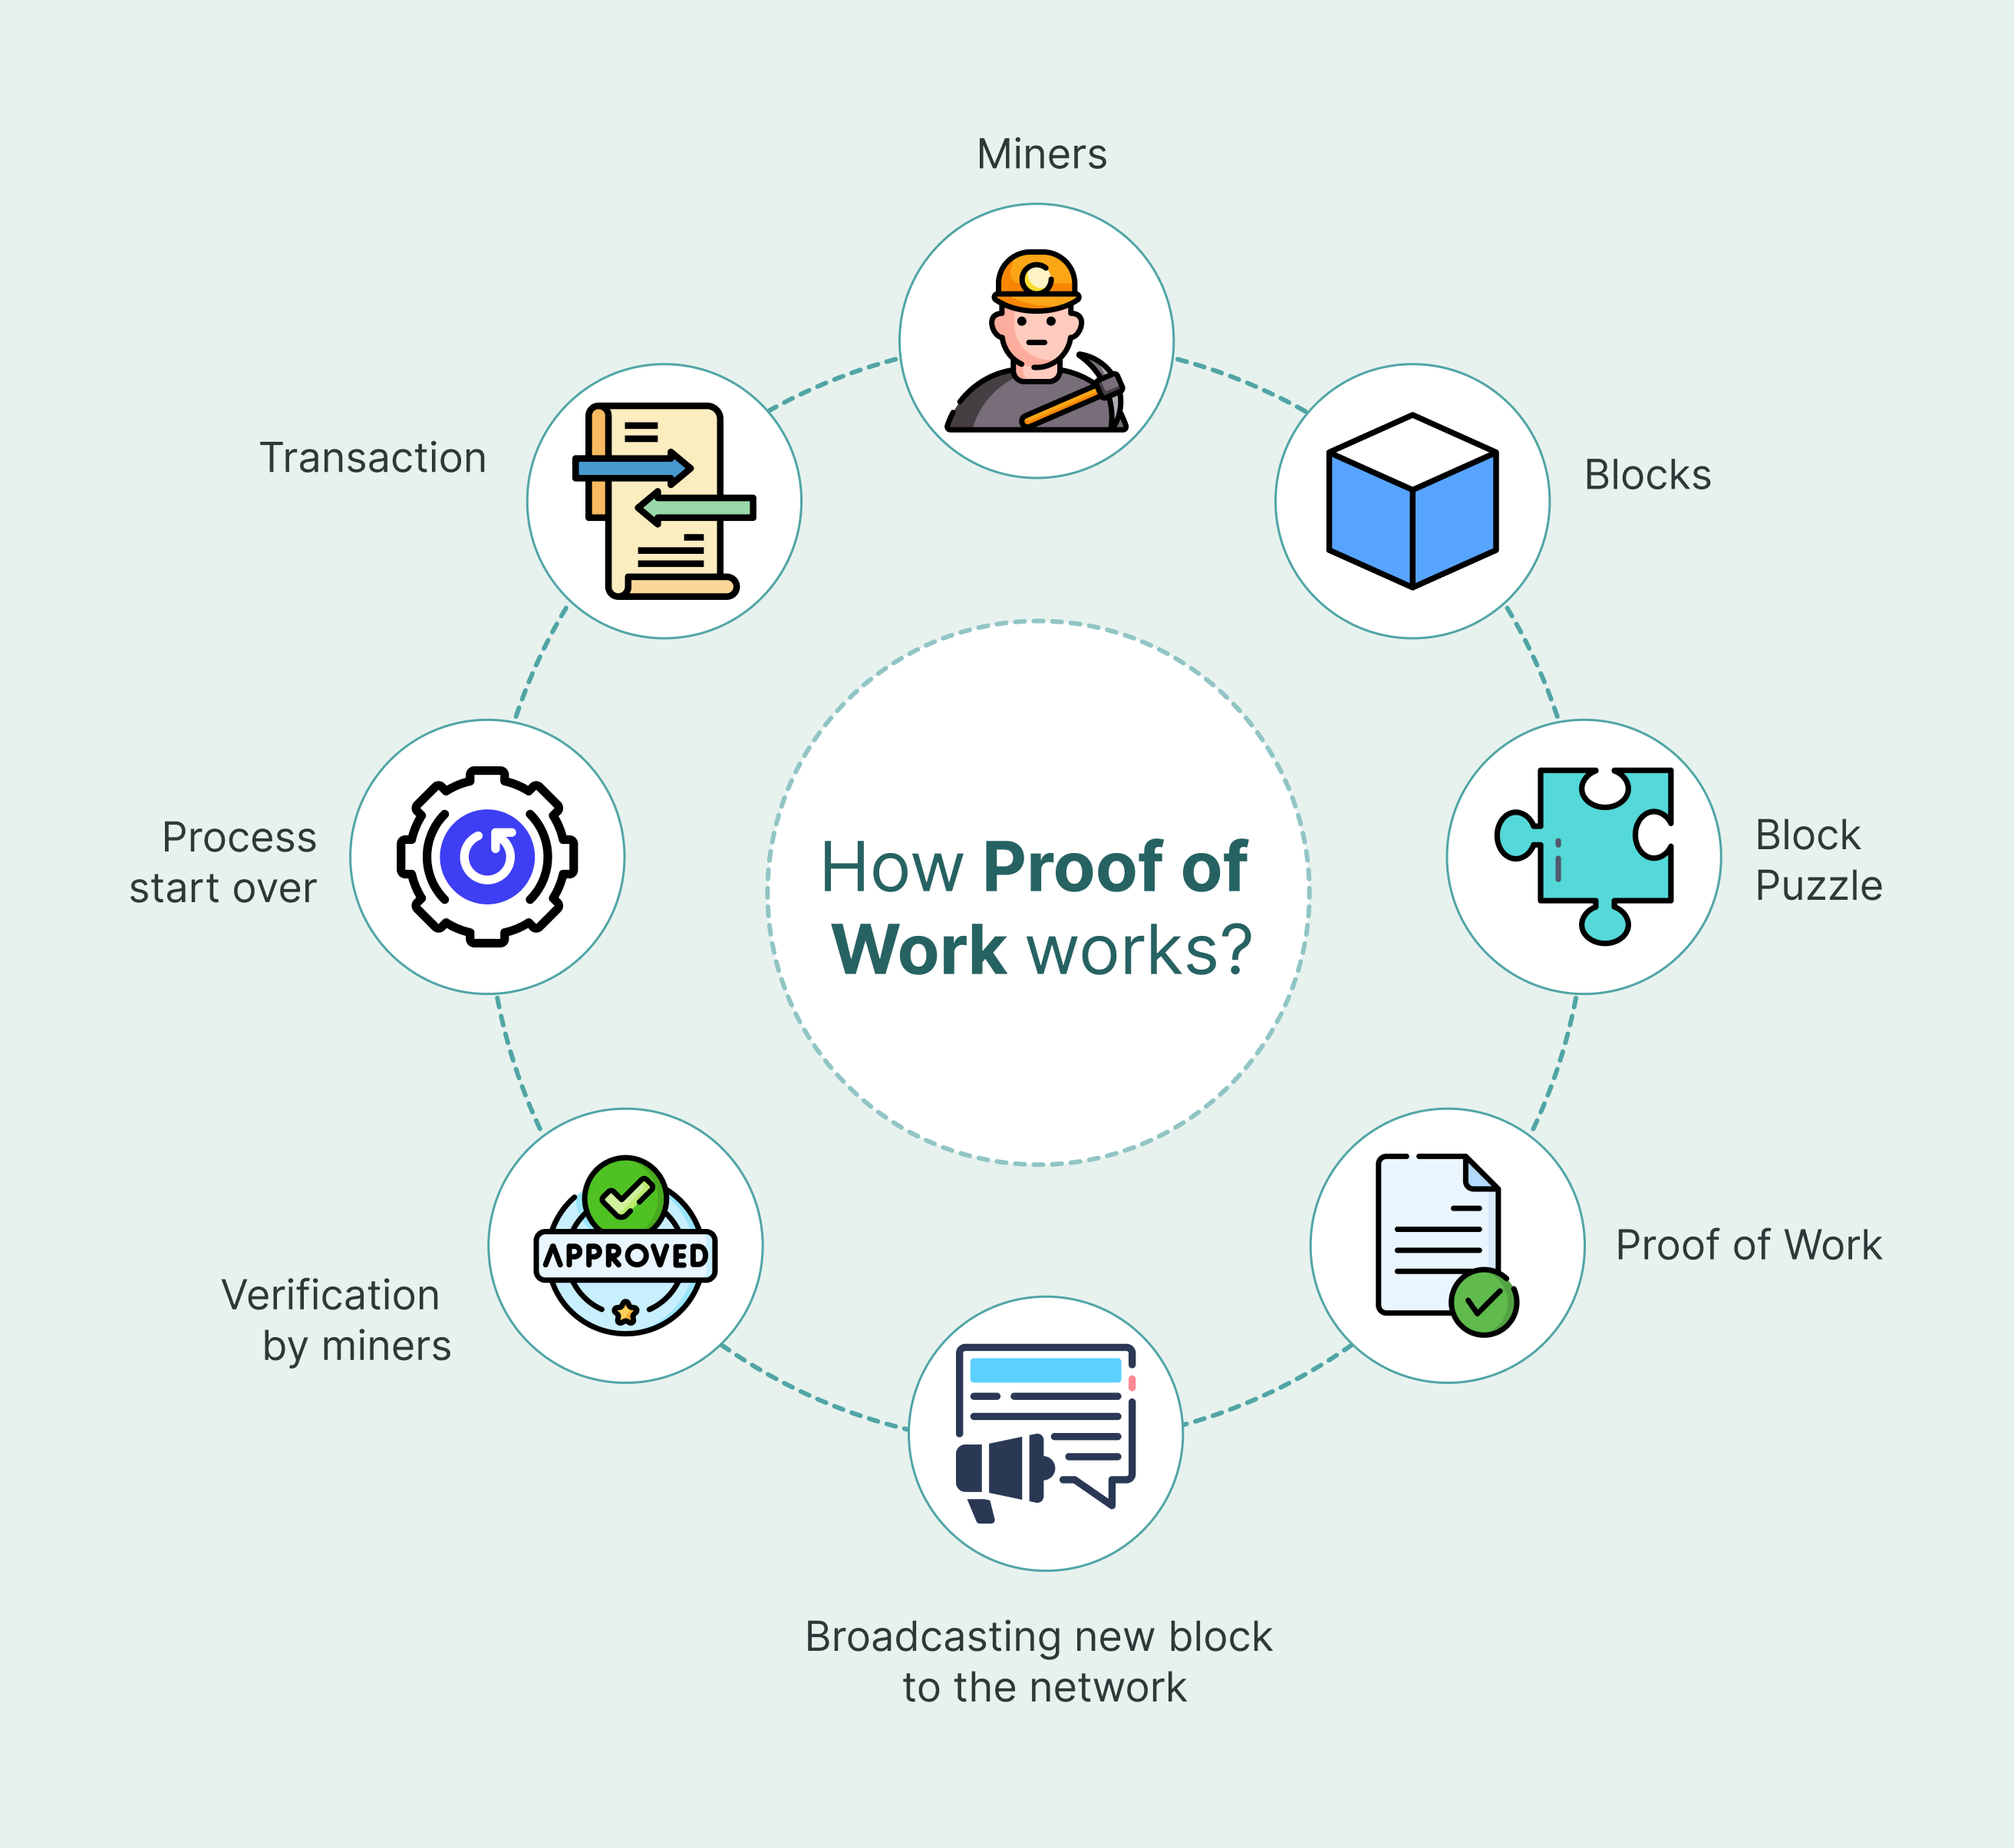
\includegraphics[width=\textwidth]{Images/ConsesnsusProofOfWork.png}
    \caption{Schemat działania Proof Of Work}
    \label{fig:ConsesnsusProofOfWork}
\end{figure}
Proof Of Stake

\vspace{1em}

Metoda konsensusu Proof Of Stake opiera się na założeniu, że im większą ktoś postawił/położył stawkę na to, że będzie mógł zostać wybrany weryfikatorem tym większe prawdopodobieństwo tego, że zostanie wybrany weryfikatorem. Szczegółowo mówiąc metoda Proof Of Stake przebiega tak, że po zebraniu odpowiedniej liczby wiadomości tworzony jest blok, lecz aby mógł on zostać utworzony najpierw weryfikatorzy decydują czy wiadomości z bloku są autentyczne i nikt ich nieautoryzowanie nie zmodyfikował. Jeśli większość weryfikatorów postanowi, żeby zbiór wiadomości jest prawidłowy tworzony jest nowy blok. Weryfikatorzy, którzy głosowali uczciwie są nagradzani za swój głos poprzez podarowanie im określonej ilości kryptowaluty (angielski – stacking), a weryfikatorzy, którzy zagłosowali nieuczciwie karani są poprzez zabranie postawionej przez nich stawki (angielski – slashing). Wydawać by się mogło, że ta metoda promuje bogatych użytkowników i umożliwia im oszustwa, lecz w rzeczywistości osoby bogate (te który postawiły najwyższą stawkę) są najbardziej odstraszane od oszustwa, ponieważ w przypadku nieuczciwego zachowania podczas weryfikacji potencjalnego bloku są oni najbardziej karani (ponieważ postawili największą stawkę). Dodatkowo ta metoda konsensus zapewnia duży stopień decentralizacji (w przeciwieństwo do tego do czego w praktyce dochodzi w Proof Of Work). W metodzie tej nie da się oszukać poprzez sytuację, że jedna osoba tworzy wiele kont (sytuacja określana też jako tworzenie multikont), ponieważ w metodzie konsensusu Proof Of Stake nie chodzi o to ilu użytkowników jest w sieci, a ile postawili oni stawki.

\vspace{1em}

Schemat obrazujący Proof of Stake:
\begin{figure}[H]
    \centering
    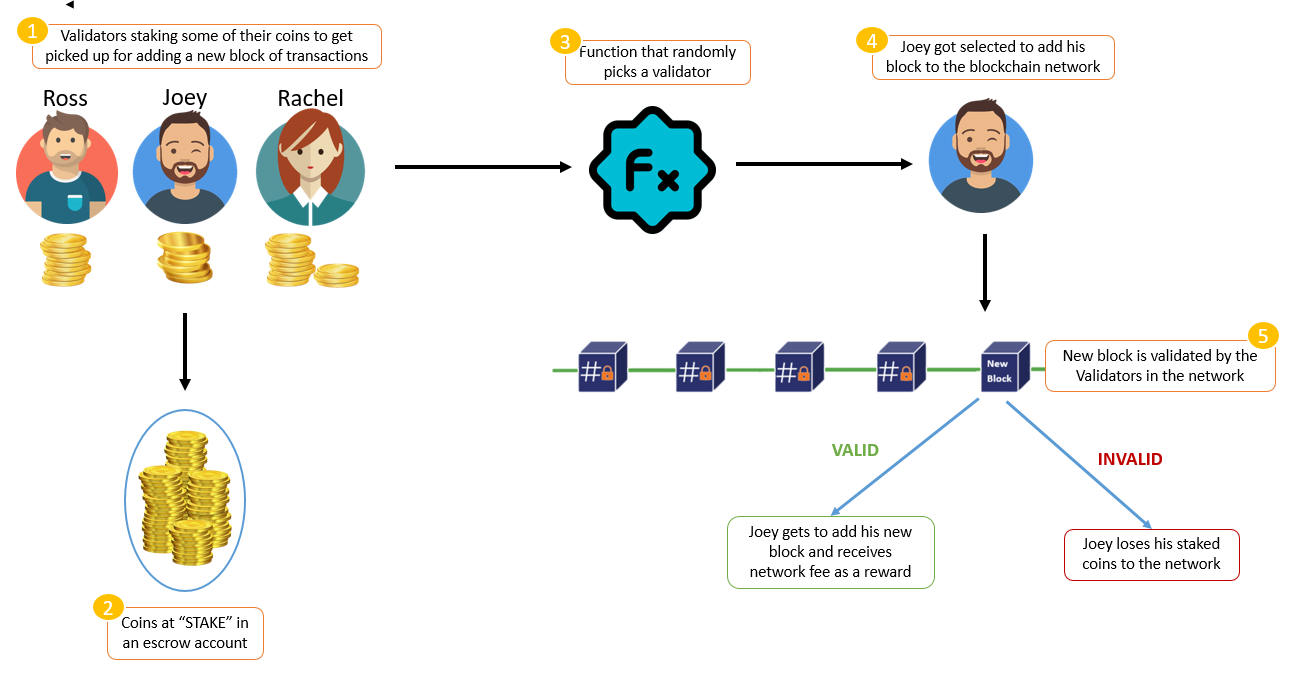
\includegraphics[width=\textwidth]{Images/ConsensusPOS.png}
    \caption{Schemat działania Proof Of Stake}
    \label{fig:ConsensusPOS}
\end{figure}
Delegated Proof Of Stake

\vspace{1em}

Delegated Proof Of Stake działa w podobny sposób jak Proof Of Stake, lecz z tym zastrzeżeniem, że wszyscy użytkownicy sieci zamiast mieć możliwość bycia wylosowanym głosują na jednego z dostępnych delegatów by on podczas weryfikacji głosował w ich imieniu. Nagrody za uczciwe głosowanie dostają delegaci, mogą podzielić się z nimi z użytkownikami, którzy na nich głosowali. Pomimo tego, że ta metoda konsensusu szybsza niż Proof Of Stake jej istotną wadą jest to, że w niej występuje o wiele większa centralizacji i zwykły użytkownik (o ile nie jest delegatem) nie ma bezpośredniej możliwości decydowania o tym czy uważa dany blok za prawidłowy czy też nie).

\vspace{1em}

Poniższy schemat ilustruje jak działa Delegated Proof Of Stake:
\begin{figure}[H]
    \centering
    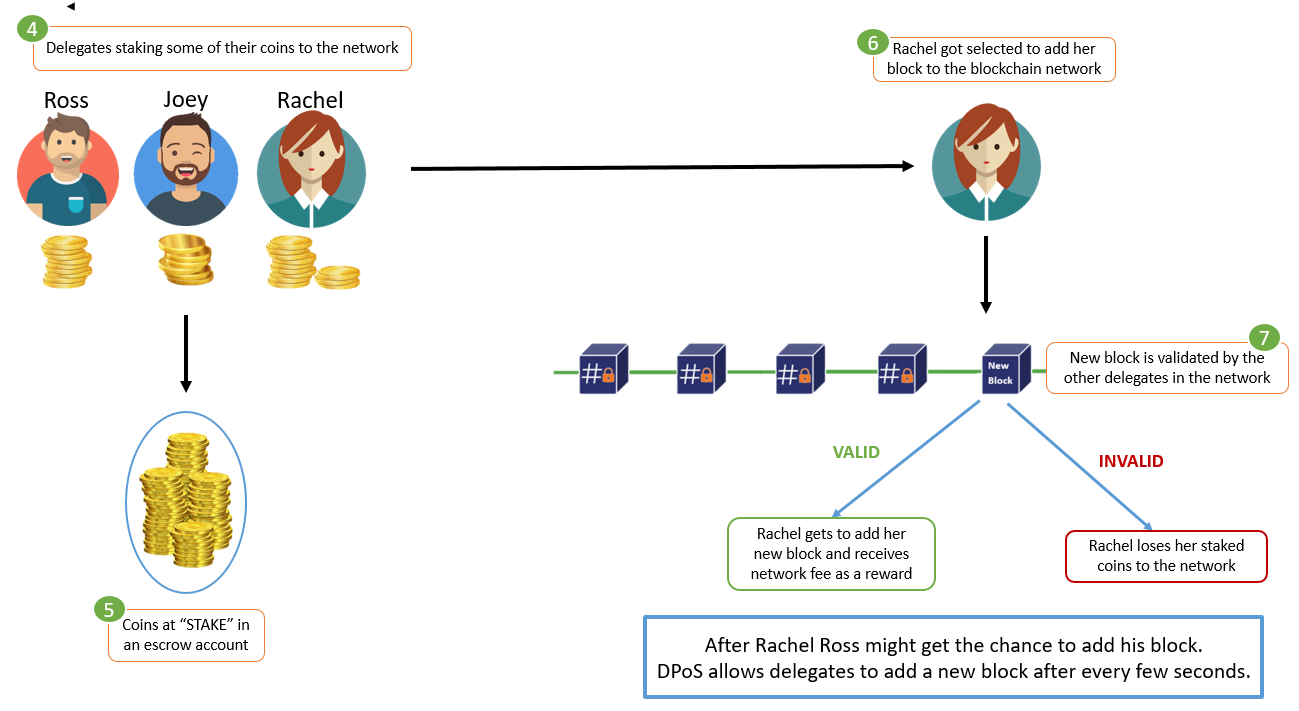
\includegraphics[width=\textwidth]{Images/ConsensusDPOS.png}
    \caption{Schemat działania Delegated Proof Of Stake}
    \label{fig:ConsensusDPOS}
\end{figure}
Proof Of Capacity

\vspace{1em}

W Proof Of Capacity każdy z uczestników posiada pliki wykresów, w których są już wcześniej obliczone wartości matematyczne. Podczas tworzenia nowego bloku ogłaszana jest pewna wartość liczbowa i uczestnicy przeszukują swoje pliki wykresów, aby znaleźć wartość najbardziej do niej pasująca. Użytkownik, który będzie miał wartości najbliżej tej poszukiwanej zostanie nagrodzony kryptowalutą. Zaletą tej metody konsensusu jest fakt, że każdy może wziąć w niej udział, ale w rzeczywistości realne szanse mają osoby o ogromnej pojemności pamięciowej, co prowadzi do tworzenia się duży grup/związków tworzonych przez różne organizacje (na przykład firmy) co prowadzi do zwiększenia i dążenie do centralizacji.

\vspace{1em}

Poniższy schemat pokazuje jak działa Proof Of Capacity:
\begin{figure}[H]
    \centering
    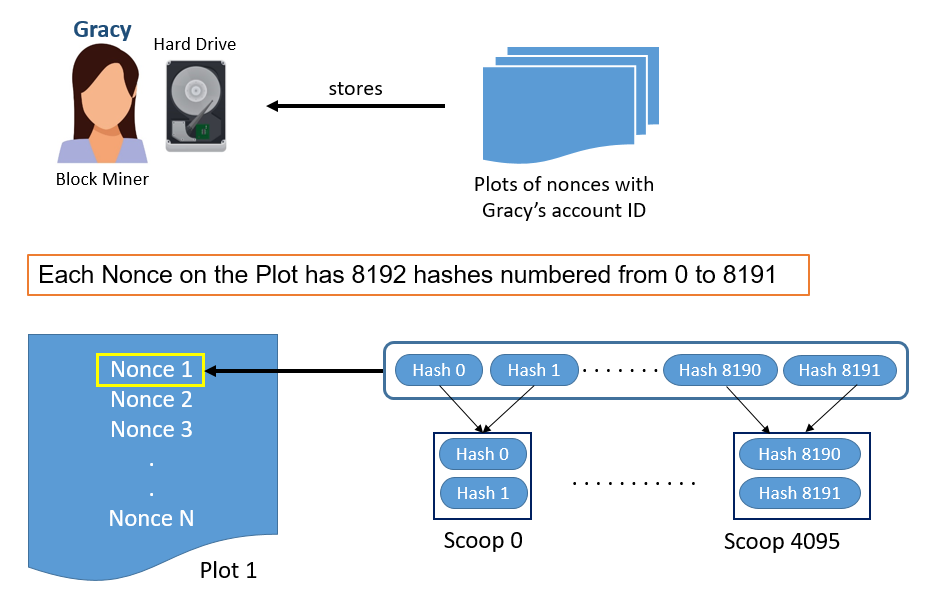
\includegraphics[width=\textwidth]{Images/ConsensusPOC.png}
    \caption{Schemat działania Proof Of Capacity}
    \label{fig:ConsensusPOC}
\end{figure}
Podsumowanie metod i uzasadnienie wyboru

\vspace{1em}

Spośród wszystkich dostępnych metod konsensusu my zdecydowaliśmy się na tą która z pozoru wydaje się być nieuczciwie faworyzującą bogatszych uczestników. Proof of Stake jest jedynym z wyżej wymienionych algorytmów, który nie ma w sobie istotnej wady jaką jest dążenie do centralizacji wywołane stosowaniem konkretnej metody konsensusu – centralizacji jednostek obliczeniowych (Proof of Work), centralizacji pojemności pamięciowej (Proof of Capacity) czy centralizacji możliwość decydowania o poprawności danego bloku jedynie dla wybranej grupy osób (Delegated Proof of Stake). Proof of Stake w przeciwieństwie z niektórymi z innych metod konsensusu nie powoduje nadmiernego zużywania zasobów – prądu używanego do obliczeń w Proof of Work i przestrzeni dyskowej (w tym sprzętu elektronicznego) by zwiększyć ilość posiadanej pamięci w Proof of Capacity. Wracając do zarzutu stawianego Proof Of Stake na początku akapitu co prawda najbogatsi (posiadający największą stawkę) mają największe szanse na zostanie weryfikatorem, ale w przypadku oszustwa są oni najmocniej karani, ponieważ tracą całą swoją postawioną stawkę (zjawisko to nazywa się slashing).
\subsection{Użycie proof of stake w praktyce}
\label{sec:POSUzycie}
\begin{lstlisting}
drawnVerifier = self.drawVerifier()
\end{lstlisting}
Przy wybieraniu osoby, która będzie mogła złożyć podpis cyfrowy w przypadku prawidłowego bloku (czy wybieraniu weryfikatora) korzysta się z funkcji, która ma go wyłonić kierując się zasadami z Proof Of Stake.
\begin{lstlisting}
def drawVerifier(self):
    personStakeList = []
    for peer in self.peers:
        personValue = {"addr": peer.addr, "port": peer.port,
        "stake": peer.stake}
        personStakeList.append(personValue)
    myValue = {"addr": ip(), "port": self.port, "stake": self.stake}
    personStakeList.append(myValue)
    personStakeList.sort(key=lambda x: x["port"])
    personSingleList = [{k: v for k, v in d.items() if k != "stake"} 
    for d in personStakeList]
    stakeSingleList = [x["stake"] for x in personStakeList]
    keyRaw = " ".join(str(x["port"]) for x in personStakeList)
    self.drawString = keyRaw
    numeric_seed = int.from_bytes(hashlib
    .sha256(keyRaw.encode('utf-8')).digest())
    random.seed(numeric_seed) #zmiana seeda dla losowania weryfikatora
    chosen_port = random.choices(personSingleList, 
    weights=stakeSingleList, k=1)[0]
    return chosen_port
\end{lstlisting}
Problemem jaki nasuwa się przy implementowaniu funkcji jest to, jak sprawić, że każdy będzie miał wylosowanego tego samego weryfikatora, mimo tego, że uruchomienia programu są niezależne od siebie. Wywołanie u każdego z użytkowników zwykłej funkcji losującej wydaje się być nasuwającym się rozwiązaniem, lecz w rzeczywistości może doprowadzić to do sytuacji, gdzie różne osoby będę uznawały różnych członków sieci za weryfikatorów, co jest sytuacją, której chcemy uniknąć. Aby rozwiązać ten problem trzeba posłużyć się niezmiennikiem jakim jest założenie, że przy dowolnej komunikacji grupowej każdy z członków jest połączony z innymi użytkownikami w grupie (na tym polega rozmowa grupowa), ta sytuacja może być chwilowo zaburzona, ponieważ, łączenie się nie zawsze występuje w tym samym czasie, ale system domyślnie dąży do tego stanu.

\vspace{1em}

Mając powyższe założenie każdy z uczestników pobiera adresy osób z którymi jest on połączony oraz swój własny, następnie co istotne te wartości są sortowane, tak aby lista w każdym wykonaniu programu (przy zawożeniu niezmiennika) była identyczna. Następnie ta lista przekształcana jest na łańcuch znaków.
\begin{lstlisting}
numericSeed = int.from_bytes(hashlib.sha256(keyRaw.encode('utf-8')).digest())
random.seed(numeric_seed)
chosen_port = random.choices(personSingleList, weights=stakeSingleList, k=1)[0]
return chosen_port
\end{lstlisting}
Dalej w kodzie z pozoru mało nieistotna funkcja skrótu, która zamienia nam łańcuch znaków na wartość liczbową jest bardzo ważna, ponieważ jeśli jest ona niedeterministyczna (dla tego samego łańcucha znaków wylosuje ona różną wartość liczbową) to w wyłanianie weryfikatora będzie mijać się z celem, bo wtedy nie wszyscy będą mieli tego samego weryfikatora. Skoro powiedziano, dlaczego deterministyczna funkcja skrótu jest tak ważna, to warto wspomnieć, że domyślna funkcja skrótu w Pythonie – hash() – nie jest funkcją deterministyczną, ponieważ wprowadzono do niej mechanizm losowości skrótu (angielski - hash randomization) który dodaje do funkcji skrótu losową ,,sól”. Z tego powodu w naszym programie zastosowano metodę hashlib.sha256(), która jest deterministyczna, ale jako wynik zwraca ciąg bajtów, więc trzeba je jeszcze przekonwertować na liczbę całkowitą.

\vspace{1em}

Następnie tak utworzoną liczbą ustawiamy ziarno generatora liczb pseudolosowych tak, aby generator dla tych samych danych wejściowych dał nam takie same wyniki. 

\begin{figure}[H]
    \centering
    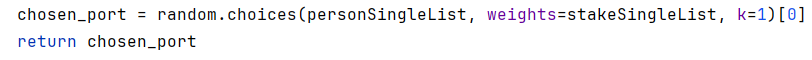
\includegraphics[width=\textwidth]{Images/CodeX10.png}
\end{figure}

Następnie w bardzo ważnym kroku który implementuje losowanie weryfikatora, jako zgodne z metodą uzyskania konsensusu Proof Of Stake jest wylosowanie jednego z uczestników, ale nie za pomocą zwykłej metody random.choice w Pythonie, która losowałaby elementy z listy z równym prawdopodobieństwem, ale z metodą random.choices, której argumentem (poza listą członków sieci), jest lista wartości postawionych przez nich jako stawki i jest ona stosowana jako lista wag, to znaczy im ktoś większą postawił stawkę, tym większa jest jego szansa na zostanie wylosowanym, co jest zgodne z założeniami Proof of Stake, jakie opisywałem wcześniej. Na koniec po wylosowaniu przekazujemy adres członka sieci, który zostanie weryfiaktorem.
\section{RSA}
\label{sec:RSA}
\subsection{Opis RSA}
\label{sec:RSAOpis}
Algorytm RSA (jest to skrót od Rivest–Shamir–Adleman) jest jednym z najbardziej popularnych i najczęściej wykorzystywanych algorytmów kryptografii asymetrycznej. W algorytmie RSA jak i w innych algorytmach użytkownik posiada parę kluczy – jest to klucz publiczny i prywatny. Klucz prywatny jest publicznie znany i nie ma żadnego problemu z jego udostępnianiem, jest generowany na podstawie klucza prywatnego. Natomiast wcześniej wspomniany klucz prywatny nie powinien być nikomu udostępniany, a jego ewentualny wyciek (czy też kompromitacja) całkowicie uniemożliwia utrzymanie komunikacji poufnej.

\vspace{1em}

Szczegółowo omawiając algorytm działa on tak, że wybiera się dwie duże liczby pierwsze, z których potem oblicza się moduł n i wartość z funkcji Eulera na podstawie tego modułu. Klucz publiczny jest liczbą względnie pierwszą do wartości funkcji Eulera. Klucz prywatny jest odwrotnością multiplikatywną wartości klucza publicznego modulo wartości funkcji Eulera.

\vspace{1em}

Przedstawia się to następującymi wzorami:
\begin{equation}
    p, \; q-losowe, \; ogromne \; liczby \; pierwsze
\end{equation}
\begin{equation}
    Obliczony \; moduł n=p*q
\end{equation}
\begin{equation}
    Obliczona \; funkcja \; Eulera \; \phi(n)=(p-1)*(q-1)
\end{equation}
\begin{equation}
    Obliczony \; klucz \; publiczny \; e \in \{NWD(\phi(n),e)=1, \; 1 \leqslant e \leqslant \phi(n)\}
\end{equation}
\begin{equation}
    Obliczony \; klucz \; prywatny \; d= e^{-1} (mod \; \phi(n))
\end{equation}
Potem, gdy chcemy zaszyfrować wiadomość odbywa się to korzystając z następującego wzoru:
\begin{equation}
    C= M^e, \; C-zaszyfrowana \;  wiadomość, \; M-oryginalny \; tekst, \; e-klucz \; publiczny
\end{equation}
Natomiast deszyfrowanie odbywa się za pomocą wzoru:
\begin{equation}
    M= C^d, \; M-deszyfrowana \; wiadmość, \;C-zakodowany \; tekst, \; d-klucz \; prywatny
\end{equation}
Bezpieczeństwo tego algorytmu opiera się na tym, że odwrócenie tych operacji i uzyskanie klucza prywatnego na podstawie czyjegoś klucza publicznego i treści zaszyfrowany i deszyfrowanych wiadomości jest obliczeniowo bardzo trudne.

\vspace{1em}

Zobrazowanie algorytmu RSA:

\begin{figure}[H]
    \centering
    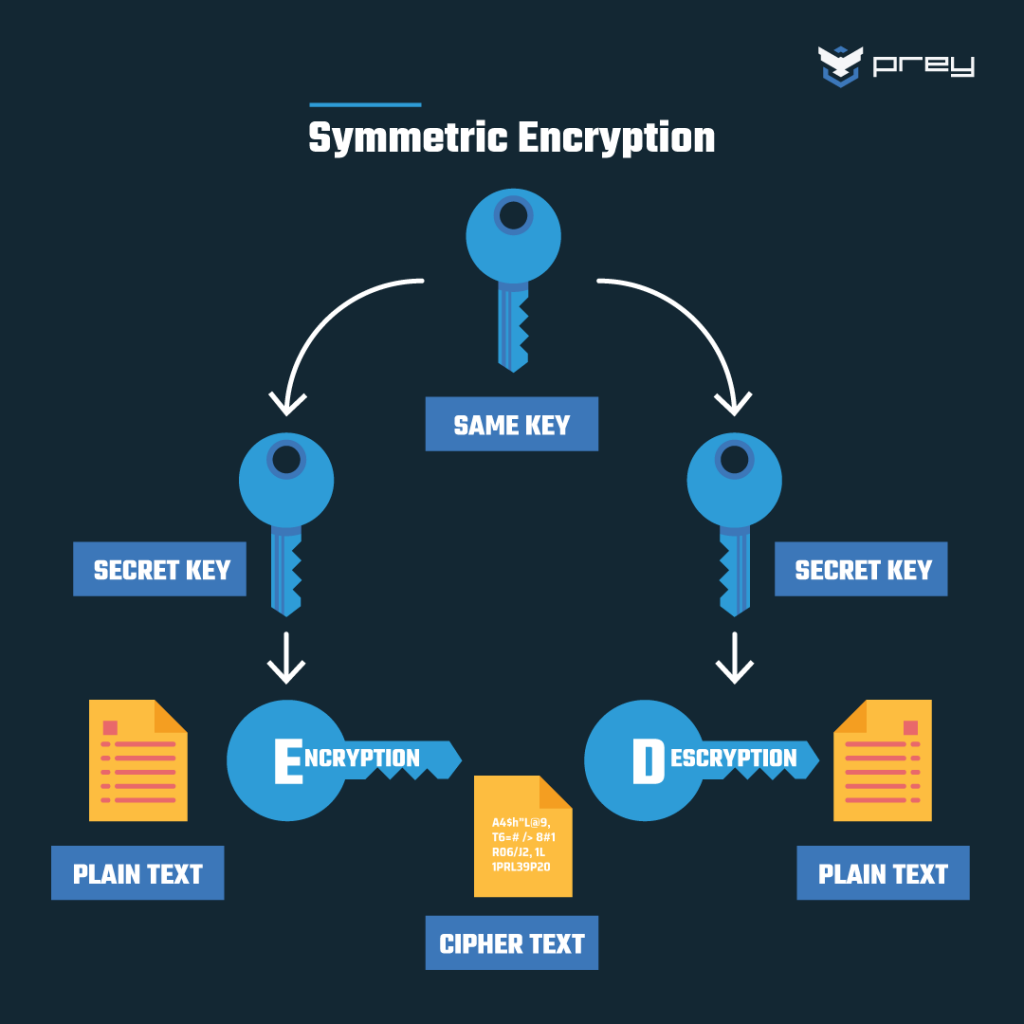
\includegraphics[width=\textwidth]{Images/RSA1.png}
    \caption{Schemat działąnia RSA}
\label{fig:RSA1}
\end{figure}

Wybraliśmy algorytm RSA, ponieważ jest on algorytmem szyfrowania asymetrycznego, który jest szeroko znany i powszechnie stosowany w praktyce. Wadami są niska wydajność i duży rozmiar kluczy, lecz są to zjawiska częste i niezbędne w kryptografii asymetrycznej dla zapewnienia bezpieczeństwa komunikacji.
\subsection{Użycie RSA w praktyce}
\label{sec:RSAPraktyka}
\begin{figure}[H]
    \centering
    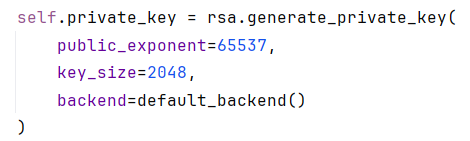
\includegraphics[width=\textwidth]{Images/CodeX11.png}
\end{figure}
Każdy z użytkowników ma generowany klucz prywatny, jest on generowany losowo i niezależnie od innych. Inni użytkownicy nie wiedzą jaki jest klucz prywatny danego użytkownika. W stosowanej przez nas implementacji wykładnik publiczny ma zalecaną wartość dosyć małej liczby pierwszej (65537), a długość klucza to 2024 bitów (to pokazuje różnicę między kryptografią asymetryczną, a kryptografią jednego klucza, gdzie jego długość w standardowych formatach AES to co najwyżej 256 bitów).
\begin{figure}[H]
    \centering
    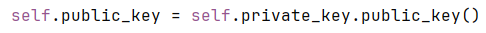
\includegraphics[width=\textwidth]{Images/CodeX12.png}
\end{figure}
Klucz publiczny jest generowany na podstawie klucza publicznego, gdyż w kryptografii asymetrycznej klucze są między sobą powiązane.
\begin{figure}[H]
    \centering
    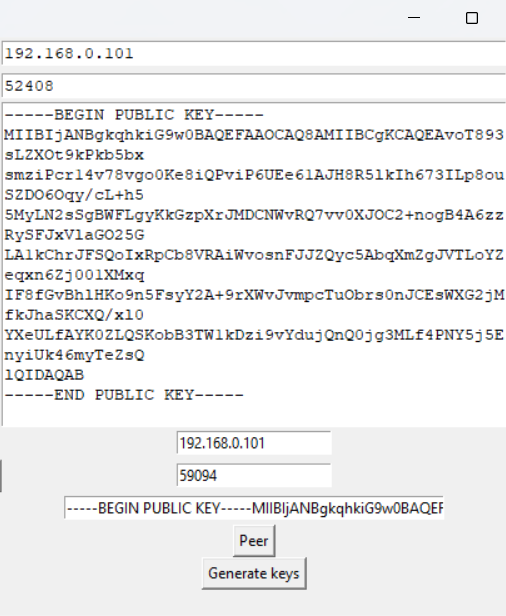
\includegraphics[width=\textwidth]{Images/CodeX13.png}
\end{figure}
Aby skutecznie połączyć się i komunikować się z innym użytkownikiem potrzebna jest znajomość jego klucza publicznego, dlatego w naszym programie przy nawiązywaniu połączenia podawany jest klucz publiczny (z którym nie ma żadnego zagrożenia bezpieczeństwa, aby został upubliczniony dla innych, w przeciwieństwie do klucza prywatnego).

\vspace{1em}

W naszym programie zmierzyliśmy się z następującym problemem, mianowicie chcemy, aby wiadomości wysyłane przez sieć były łatwo dostępne dla innych użytkowników, którzy są członkami sieci, ale żeby ich treść nie była dostępna dla osób z zewnątrz (nie można ich przesyłać przez sieć jako zwykły tekst, ponieważ wtedy istniałaby możliwość podsłuchania i zostałby zaburzony jeden z filarów naszego systemu, czyli poufność wiadomości). Z tego powodu zadecydowaliśmy do szyfrowania wiadomości w sposób symetryczny (będzie ono opisane w innym akapicie, warto wiedzieć, że jest zdecydowanie szybsze od asymetrycznego). Teraz pojawia się problem czym będzie klucz w szyfrowaniu z pojedynczym kluczem i jak go ustalić w sposób bezpieczny. Tu jako rozwiązanie pojawia się szyfrowanie asymetryczne.

\begin{figure}[H]
    \centering
    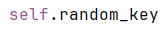
\includegraphics[width=\textwidth]{Images/CodeX135.png}
\end{figure}

Każdy z użytkowników generuje losowy klucz sesyjny i w momencie powiększania się grupy (dodania nowego użytkownika) lub jej się zmniejszenia (usunięcie jednego z użytkowników) klucz sesyjny generuje się na nowo.

\begin{figure}[H]
    \centering
    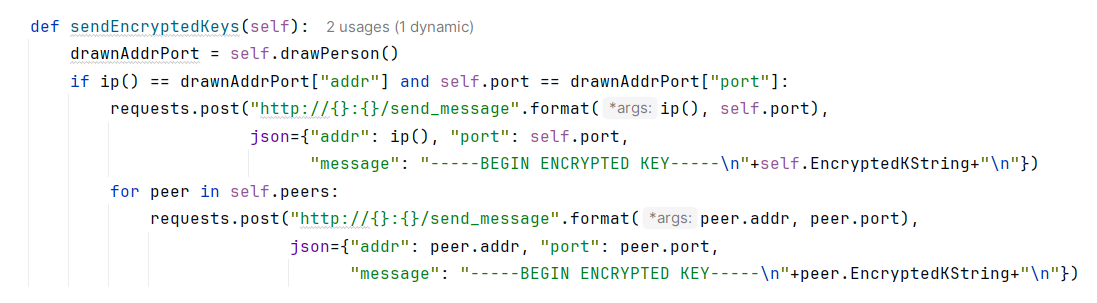
\includegraphics[width=\textwidth]{Images/CodeX14.png}
\end{figure}

Potem jeden z użytkowników jest w momencie zmiany składu grupy wybierany jako osoba mająca rozesłać klucz sesyjny.

\begin{figure}[H]
    \centering
    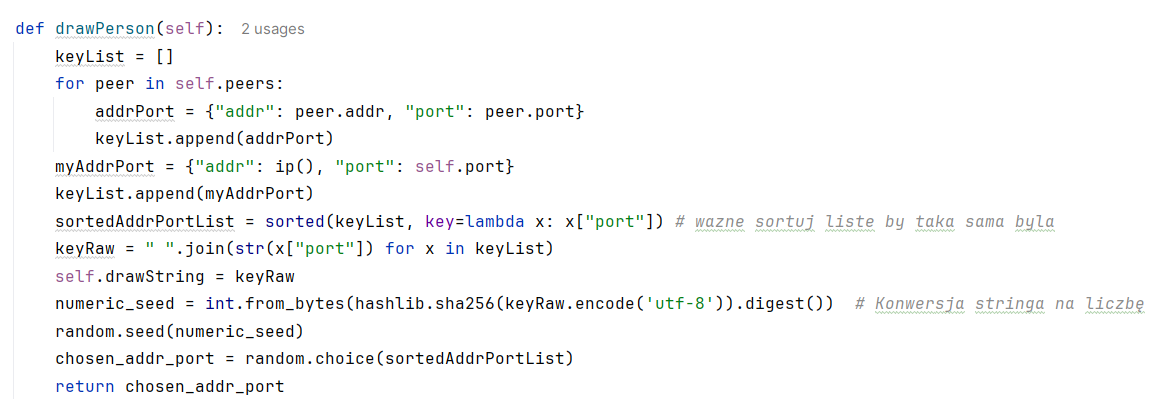
\includegraphics[width=\textwidth]{Images/CodeX15.png}
\end{figure}

Tak samo jak w przypadku Proof Of Stake mechanizm losowania osoby mającej wysyłać klucz sesyjnym innym musi być taka sama dla wszystkich, tak oby osoba wysyłająca była w każdej instancji programu taka sama, inaczej użytkownicy mieliby różne klucze sesyjne co uniemożliwiłoby komunikację. Tak samo jak w Proof Of Stake tworzymy listę użytkowników, którą następnie sortujemy, aby każdy program miał ją w takiej samej postaci. Potem listę zamieniamy na łańcuch znaków i używając deterministycznej funkcji skrótu (zwracającej te same wyniki dla tych samych danych) hashlib.sha256 (a nie na przykład domyślnej funkcji hash() w Pythonie, która nie jest deterministyczna) uzyskujemy wartość, która będzie ziarnem dla generatora liczb losowych i następnie wylosowany przez ten generator użytkownik (za pomocą standardowej funkcji random.choice()) będzie taki sam we wszystkich instancjach programu.

\begin{figure}[H]
    \centering
    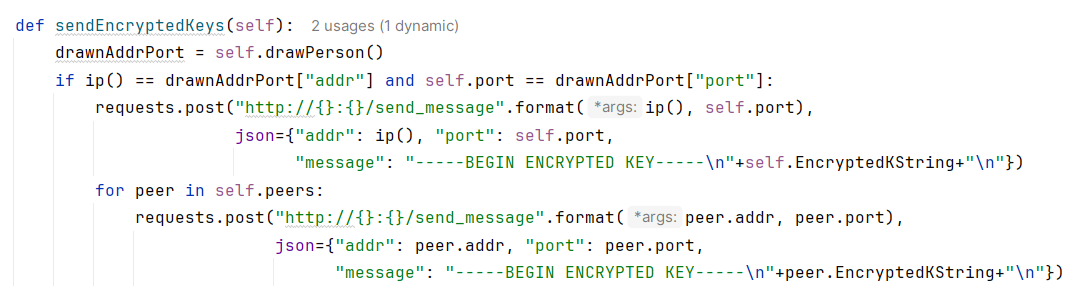
\includegraphics[width=\textwidth]{Images/CodeX16.png}
\end{figure}
\begin{figure}[H]
    \centering
    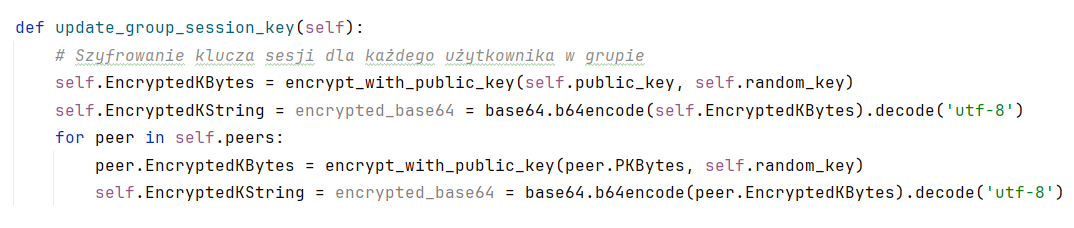
\includegraphics[width=\textwidth]{Images/CodeX17.png}
\end{figure}
Następnie po wylosowaniu osoby będącej odpowiedzialną za wysyłanie klucza ta osoba rozsyła do siebie klucz sesyjny zaszyfrowany swoim własnym kluczem publicznym, a do innych osób w sieci (biorąc pod uwagę niezmiennik, że każdy z każdym w danej grupie jest połączony) rozsyła klucz sesyjny zaszyfrowany kluczem publicznym danej osoby (właśnie dlatego, przy nawiązywaniu połączenia klucz podawany jest klucz publiczny – inaczej nie dało by się przekazać innym klucza sesyjnego z zachowaniem poufności). Dodatkową informacją godną uwagi jest fakt, że przy wysyłaniu innym zakodowanego klucza sesyjnego jest on poprzedzany nagłówkiem w celu łatwiejszego odebrania przez adresatów wiadomości.
\begin{figure}[H]
    \centering
    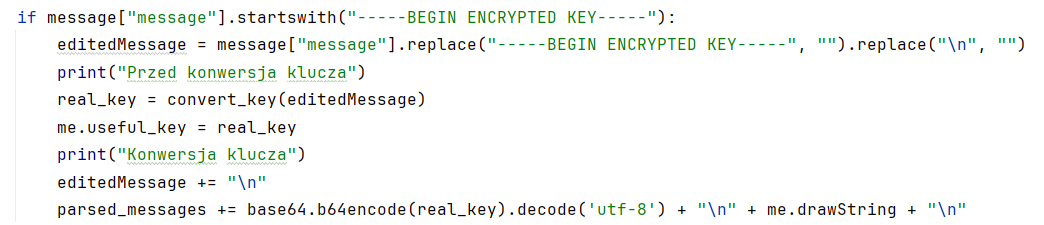
\includegraphics[width=\textwidth]{Images/CodeX18.png}
\end{figure}
Każdy z odbiorców po otrzymaniu wiadomości usuwa z niej nagłówek i tworzy z niej klucz za pomocą funkcji konwertującej klucz sesyjny zakodowany przez klucz publiczny w formacie Base64 na użyteczny klucz sesyjny stosowany do kryptografii pojedynczego klucza.
\begin{figure}[H]
    \centering
    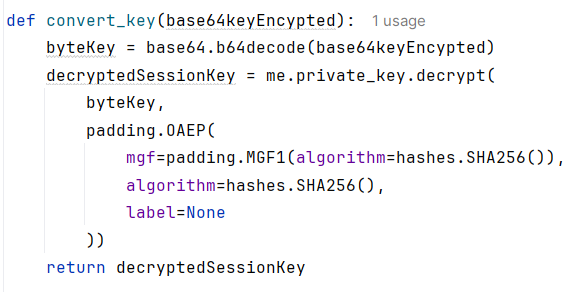
\includegraphics[width=\textwidth]{Images/CodeX19.png}
\end{figure}
W funkcji konwertującej zaszyfrowany w formacie Base64, pierwszą operacją jest zamienienie z typu łańcuchu znaków na format ciągu bajtów. Potem przebiega typowa dla kryptografii asymetrycznej operacja deszyfrowania kluczem prywatnym danego użytkownika, jednak szczególnie ważnym w niej jest fakt, że jest ona deterministyczna dla tych samych danych wejściowych do odszyfrowania, co oznacza, że jeśli podamy klucz sesyjny zaszyfrowany kluczem publicznym danego użytkownika i odszyfrujemy go jego kluczem prywatnym to zawsze wyjdzie nam poprawny klucz sesyjny z początku procesu. Ten klucz będzie potem wykorzystywany do odszyfrowania pojedynczych wiadomości w bloku przy wykorzystywaniu kryptografii klucza tajnego (dokładniej algorytmu AES, o którym jest mowa w innym akapicie).
\section{AES}
\label{sec:AES}
\subsection{Opis AES}
\label{sec:AESOpis}
Algorytm AES (skrót od Advanced Encryption Standard) jest jednym z najbardziej znanych algorytmów kryptografii symetrycznej. Jego zdecydowaną zaletą jest fakt, że ten algorytm jest dobrze przetestowany i powszechnie używany. Jego historia opiera się na tym, że wcześniej powszechnie używany algorytm DES (Data Encryption Standard) nie zapewniał już odpowiedniego poziomu bezpieczeństwa, między innymi przez krótką długość klucza i małą długość bloku co powodowało niską odporność na ataki. W konkursie ogłoszonym przez NIST (skrót od National Institute of Standards and Technology) mającym zastąpić DES wygrał algorytm, którego oryginalna nazwa brzmiała Rijndael. Aby zrozumieć, dlaczego AES został wybrany i jest tak powszechnie stosowany warto przyjrzeć się jak działa i zobaczyć jego charakterystyczne cechy.

\vspace{1em}

Tak jak wcześniej wspomniałem AES jest algorytmem szyfrowania symetrycznego, który opiera się na blokach. Mają one stały rozmiar 128 bitów. Cały algorytm opiera się na wielu matematycznych operacjach, które są podzielone na rundy. To, ile jest rund zależy od tego jaka jest długość (10 rund dla klucza 128-bitowego, 12 rund dla klucza 192-bitowego, 14 rund dla klucza 256-bitowego). Operacje są wykonywane na macierzach 4x4 bajty.

\vspace{1em}

Operacje wykonywane w każdej z rund przedstawiają się następująco:
\begin{enumerate}
    \item Zamiana bajtów – zamiana każdego bajtu według schematu w tabeli podstawień, ma to na celu to, żeby te operacje były nieliniowe,
    \item Zamiana wierszy – przesunięcie określonej ilości wierszy macierzy, w celu dyfuzji danych
    \item Mieszanie kolumn – jest to osiągnę przez mnożenie elementów tych kolumn
    \item Dodanie klucza – do macierzy dodawany jest klucz rundowy (głównie przez wykorzystanie operacji alternatywy rozłącznej)
\end{enumerate}
Wszystkie te operacje mają na celu zaciemnienie oryginalnych danych tak, żeby nie dało się ich odszyfrować bez znajomości symetrycznego klucza, a fakt, że operacje są wykonywane w wielu rundach czyni algorytm jeszcze bardziej trudniejszym do złamania.

\vspace{1em}

Ilustracja działania AES:
\begin{figure}[H]
    \centering
    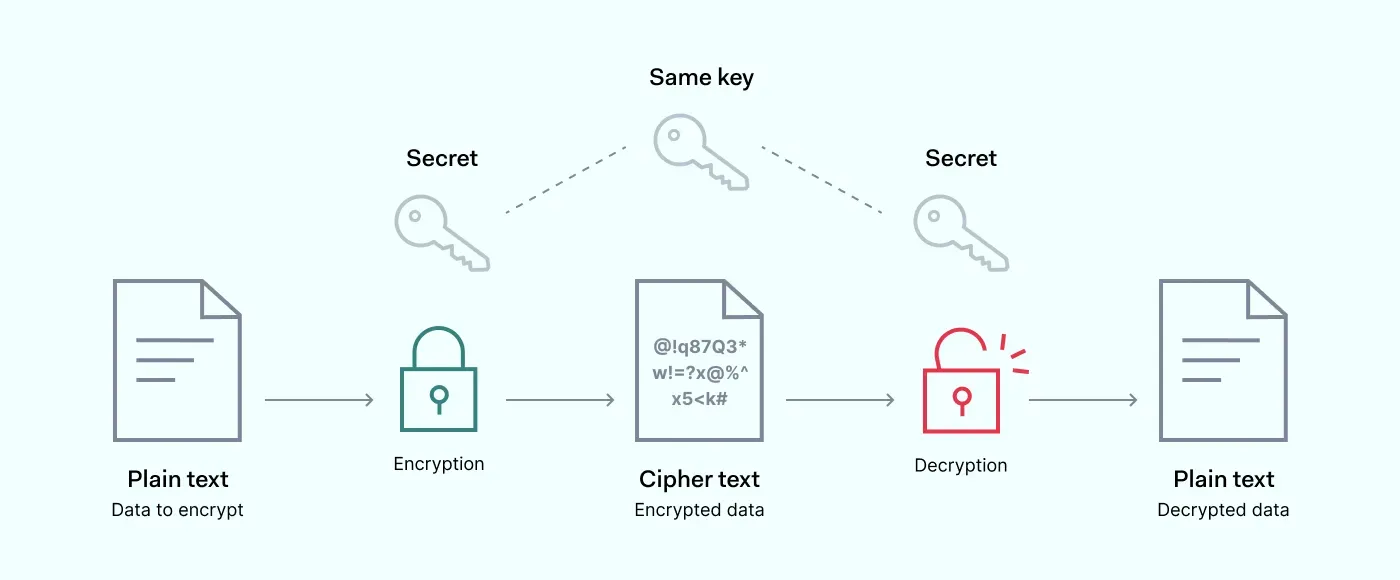
\includegraphics[width=\textwidth]{Images/AES1.png}
    \caption{Schemat działania AES}
    \label{fig:AES1}
\end{figure}
Z innych zalet oprócz bezpieczeństwa i odporności na złamanie szyfru, o których zostało wspomniane wcześniej inną cechą algorytmu Rijndael jest jego wydajność, w porównaniu do innych algorytmów szyfrowania symetrycznego (w porównaniu do algorytmów szyfrowania asymetrycznego oczywiście też, ale kryptografia klucza publicznego jest kilka rzędów wolniejsza od kryptografii z jednym kluczem). Między innymi to wydajność Rijndael (bezpieczeństwo oczywiście też) była cechą, która sprawiła, że został on wybrany nad algorytmami Serpent, Twofish, RC6 i MARS. Algorytmy te same w sobie również były bezpieczne, ale ich gorsza wydajność sprawiła, że to nie one zostały w 2001 wybrane przez National Institute of Standards and Technology na następcę DES. Inną ważną cechą AES jest jego powszechne stosowanie i popularność, jest on między innymi wykorzystywany w protokołach TLS (Transport Layer Security), IPsec (Internet Protocol Security) czy WPA (WiFi Protected Access).
\subsection{Użycie AES w praktyce}
\label{sec:AESPraktyka}
\begin{figure}[H]
    \centering
    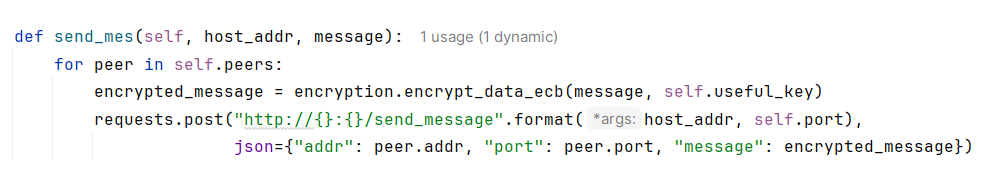
\includegraphics[width=\textwidth]{Images/CodeX20.png}
\end{figure}
W powyższej funkcji dane zanim będę przesłane innym członkom sieci, są najpierw szyfrowane za pomocą klucza symetrycznego (dokładnie mówiąc, jest to klucz sesyjny, jak on powstaje zostało pokazane w akapicie opisującym algorytm RSA).
\begin{figure}[H]
    \centering
    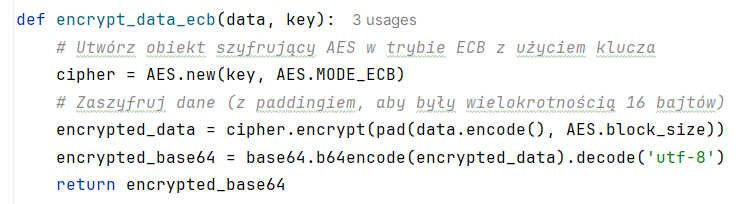
\includegraphics[width=\textwidth]{Images/CodeX21.png}
\end{figure}
Samo szyfrowanie danych odbywa się przez funkcję encryptDataEcb, której parametrami są tekst podany do zaszyfrowania oraz klucz sesyjny. W samej funkcji najpierw tworzony jest obiekt szyfrujący AES, który jest ustawiony w trybie wiązania bloków zaszyfrowanych ECB - Electronic CodeBook. Dlaczego akurat w takim trybie a nie na przykład CBC (Cipher Block Chaining) czy CFB (Cypher Feed Back)? Powodem jest użyteczność naszej funkcji, chcemy, aby była ona deterministyczna, co wyklucza elementy losowe, a ECB jako jedyny z powszechnie używanych trybów wiązania bloków zaszyfrowanych nie korzysta z losowych wektorów inicjalizujących. Następnie szyfrujemy z wykorzystaniem wcześniej stworzonego obiektu szyfrującego, a wynik tej operacji przekonwertowujemy do łańcucha znaków za pomocą Base64.
\begin{figure}[H]
    \centering
    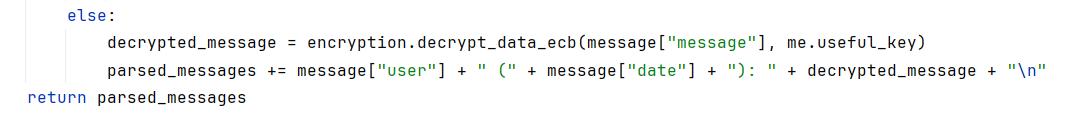
\includegraphics[width=\textwidth]{Images/CodeX22.png}
\end{figure}
Jeśli otrzymane przez użytkownika dane nie są poprzedzone żadnym nagłówkiem (na przykład oznaczającym przesłanie klucza) to oznacza, że jest to zwykła zakodowana wiadomości i przeprowadzana będzie na niej operacja deszyfrowania za pomocą funkcji decryptDataEbc.
\begin{figure}[H]
    \centering
    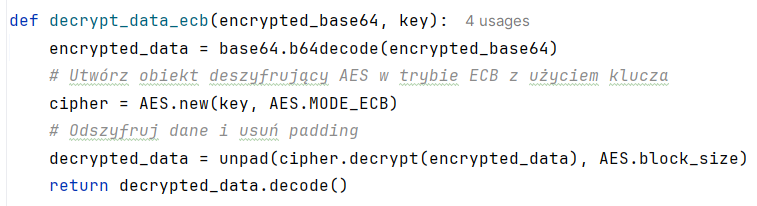
\includegraphics[width=\textwidth]{Images/CodeX23.png}
\end{figure}
W funkcji deszyfrującej najpierw zaszyfrowane dane konferujemy z formatu Base64 na ciąg bajtów, potem podobnie jak w operacji szyfrowania tworzymy nowy obiekt szyfrujący, którego tryb wiązania bloków zaszyfrowanych to ECB. Następnie deszyfrujemy dane i usuwamy zbędne wypełnienie.